\chapter{Future Work}
\label{chapter:futurework}

\begin{changemargin}{1.0cm}{1.0cm} 
\abstractpreamble{At a certain point, work on various codes developed in this work, as well as the resulting Fe-Pd potential(s) had to stop, but there are a number of improvements that could be made given more time.}
\end{changemargin}


\section{Activity Code}

\subsection{Experimental Activity Readings for Ion Irradiated Targets}

The Activity code was developed using data from the \acrshort{tendl} data file.  To test the validity of the code, an Iron sample was irradiated and its activity was measured several days after irradiation.

To validate the code further, a range of pure targets and alloys would be irradiated by a cyclotron, with targets of varying thickness and beams of varying fluences and energies.  This would generate data to be used to compare to the results predicted by the code.  


\subsection{Code Improvements}

Ideally, a built in ion transport code similar to \acrshort{srim} would be developed.  Failing this, an improvement in the reaction rate calculation and a rewrite of the code in Python with F2PY to improve ease of developing in the future.

Given the variation of energy ranges between cross section databases, it would be useful to give the user a selection of a variety of \acrshort{tendl} and similar data files to choose from.  In addition to this, reaction cross sections could be computed over a set energy range using the TALYS code specifically for use in the Activity program.

Finally, extending the range of projectiles in the Activity code to include Deuterons, Tritons and Helium would be useful as the cyclotron is capable of accelerating these particles as well as protons.  It would require an extension of the database to include the relevant cross section files.


\section{Potential Fitting and MD Simulations}

Two potentials were derived for Fe-Pd that reproduced the bulk properties of each element individually reasonably well.  Cohesive energy and surface energy plots could be improved by adding new modules to help fit the potential, and overall more \acrshort{dft} data could be collected.

\subsection{Larger Supercells}

In many examples in the literature, the supercell sizes were at least 4x4x4 containing 256 atoms for \acrshort{fcc} crystals.  These require much more memory and processing power, especially considering the lack of symmetry and inclusion of magnetism in the calculations.  More calculations over a greater range of randomised atom locations, with a varying percentage of palladium (1 atom per 256, 2 atoms per 256, 3 atoms per 256 and so on) would also help towards fitting a better potential.

\subsection{Properties of Fe-Pd Alloy}

The properties of palladium were known and those of pure FCC iron were calculated.  Using \acrshort{dft} to calculate the properties of a 1-2\% iron-palladium alloy would provide another set of data to fit the potentials to.


\FloatBarrier
\subsection{Improved Fitting: Surface Energy, Cohesive Energy and Defects}

The cohesive energy and surface energy plots for the derived iron and palladium potentials were recognisable, but they were not smooth and did have many small bumps in the plots.  Having plotted the same for Aluminium, the \acrshort{dft} results were much smoother.  

\begin{figure}[h]
\begin{minipage}[b]{0.48\linewidth}
  \begin{center}
    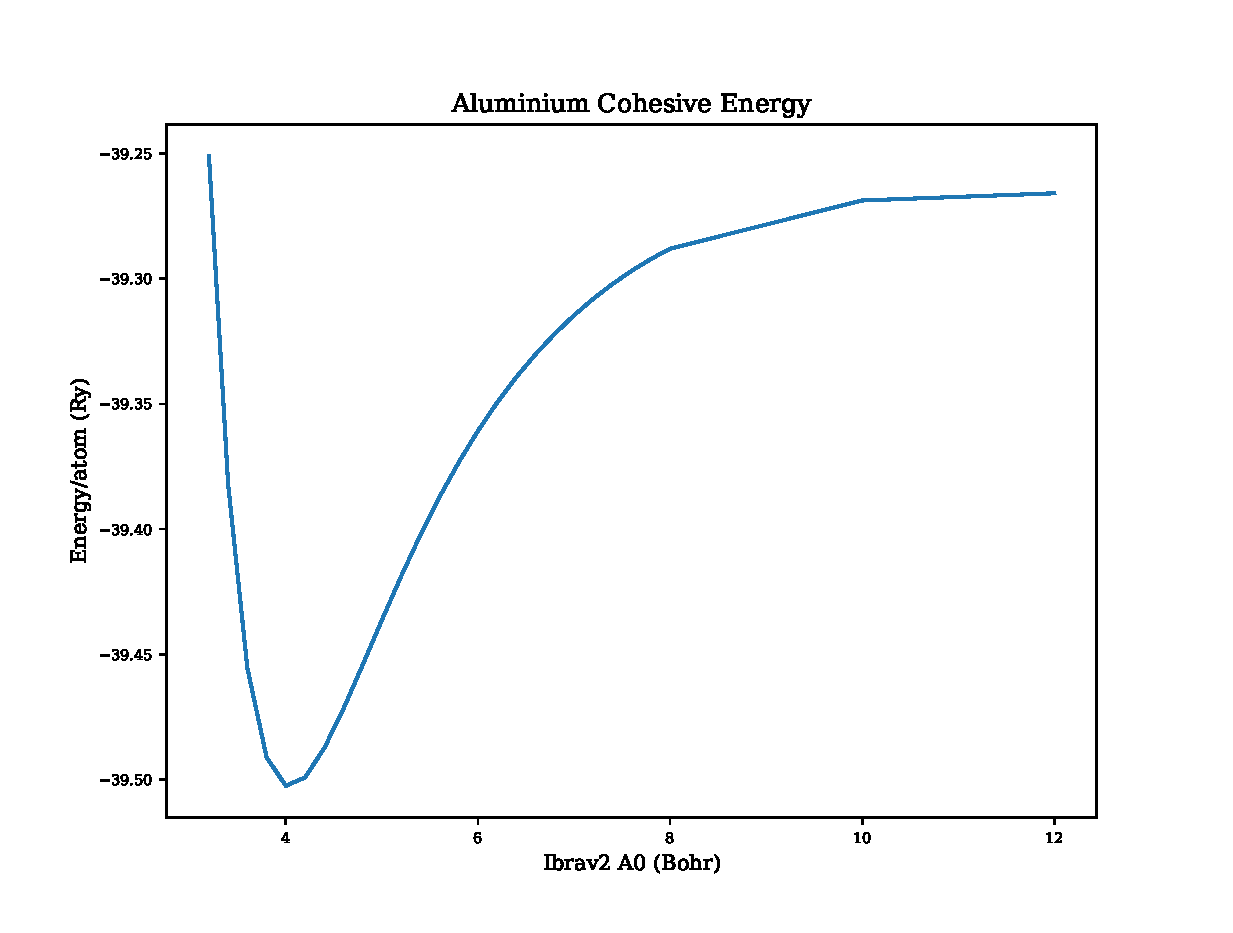
\includegraphics[width=.98\linewidth]{chapters/future_work/plots/al_cohesive_energy.eps}
    \caption{DFT Aluminium Cohesive Energy}
    \label{fig:dftaluminiumcohesive}
  \end{center}
\end{minipage}
\begin{minipage}[b]{0.48\linewidth}
  \begin{center}
    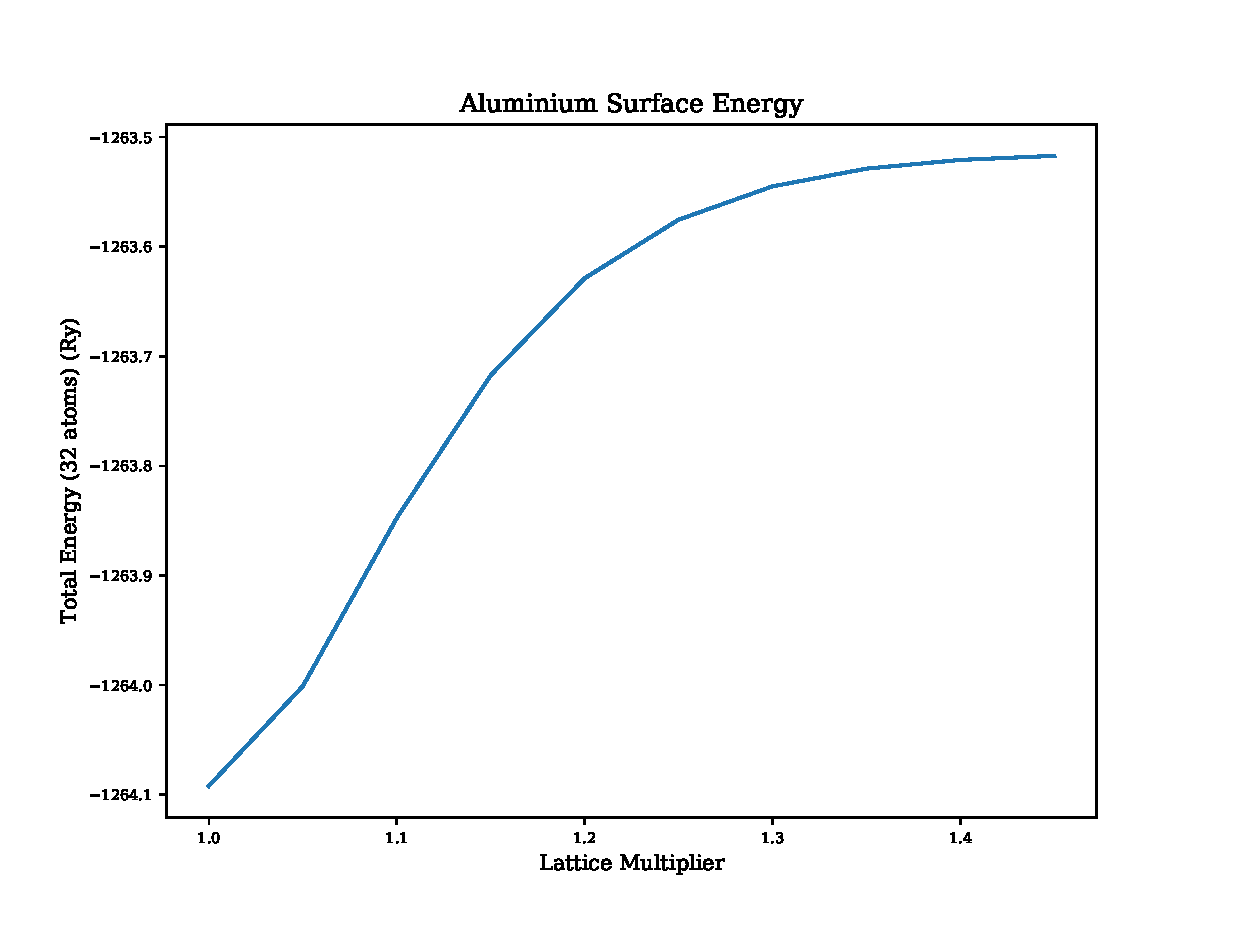
\includegraphics[width=.98\linewidth]{chapters/future_work/plots/al_surface_energy.eps}
    \caption{DFT Aluminium Surface Energy}
    \label{fig:dftaluminiumsurface}
  \end{center}
\end{minipage}
\end{figure}


Rather than just fit the data to the energy surface, it would be to useful to create DFT configurations for the cohesive energy and surface plots for both Iron and Palladium.  These configurations, and the energies, forces and stresses computed by \acrshort{dft} would be used to improve the fitting process.

Currently the fitting code has two modules: EFS, to compute energy, forces and stress of a set of atom configurations provided and BP, to calculate the material properties (bulk modulus, elastic constants etc).  A new module could be created to calculate the value of the surface energy.  It would require computing the relaxed energy of the potential for the bulk material.  Next a slab, with enough vacuum along its surface(s) to prevent interference over the periodic boundary condition, would have the atomic positions relaxed and the energy (for the potential) calculated.  This would allow computation of the value of the surface energy to be used to improve the potential.

The computation of the cohesive energy could also be implemented into a module.  The relaxed bulk energy would be computed as well as that of isolated atoms, and this would give enough data to compute the cohesive energy.

Finally, a defects module could be created.  Common defects, and their experimental or \acrshort{dft} computed energies, would be provided by the user.  The module would create the configurations based on the user's input.  The volume and positions of the atoms would need to be relaxed with the current iteration of the potential for each defect, and the energy computed.  This, with the energy in bulk, would compute the energy of each defect.


\subsection{Improved Potential: Non-Isotropic Structure}

With a collinear spin-polarized \acrshort{dft} calculation, the relaxed structure was slightly longer in the y direction.  Investigating the use of an angularly dependent potential might be worthwhile and the \acrshort{meam} type potential with an angularly dependent electron density would be a starting point (section \ref{section:meam}).

\subsection{Improved Potential: Fe-Ni-Cr-Pd}

Given more time and a larger computer, more complicated \acrshort{dft} calculations could be performed that better represent the material, austenitic stainless steel.  1\% palladium doped steel could be represented as a 4x4x4 supercell containing 256 atoms.  For \gls{304SS} approximately 50 chromium, 25 nickel, 178 iron and 3 palladium atoms would be needed (and small variations on these figures).


